\documentclass{article}

\usepackage{float}
\usepackage{graphicx}
\usepackage{algorithm}
\usepackage[utf8]{inputenc}
\usepackage[noend]{algpseudocode}

\title{Algoritmos - Lab3}
\author{Santiago Álvarez Sepúlveda }
\date{Octubre 8 2018}

\begin{document}

\maketitle

\section{Assume that A is an array of size  n of  distinct elements}

\subsection{Mínimo Número de Inversiones - Instancias}
Dado el arreglo $A$ que contiene $N$ elementos distintos, el mínimo número de inversiones que ocurriran al utilizar un algoritmo de ordenamiento, acontece cuando los elementos del arreglo se encuentran previamente ordenados, esto es cuando:

\begin{equation}
    A = \{A_i | A_i < A_j \leftrightarrow i < j \forall i, j = 0, 1, ..., N-1\}
\end{equation}

\subsection{Máximo Número de Inversiones - Instancias}
Dado el arreglo $A$ que contiene $N$ elementos distintos, el máximo número de inversiones que ocurriran al utilizar un algoritmo de ordenamiento, acontece cuando los elementos del arreglo se encuentran totalmente  desordenados, es decir en el orden contrario, esto es cuando:

\begin{equation}
    A = \{A_i | A_i > A_j \leftrightarrow i < j \forall i, j = 0, 1, ..., N-1\}
\end{equation}


\subsection{Complejidad (peor caso de comparaciones) de Brute Force Counting sobre A}

\begin{algorithm}[H]
    \caption{Insertion Sort Descendente}\label{alg:isort_desc}
    \begin{algorithmic}[1]
        \Procedure{BruteForce}{$A$}
            \State $count = 0$
            \For{$i=1$ to $A$.length}
                \For{$j=i$ to $A$.length}
                    \If {$A[i] > A[j]$}
                        \State $count \gets count + 1$
                    \EndIf
                \EndFor\label{isort_for}
            \EndFor\label{isort_for}
            \State $return count$ 
        \EndProcedurelatex algorithm 
    \end{algorithmic}
\end{algorithm}

\subsection{Complexity (worst case number of comparisons) of the divide an conquer (mergesort) counting on A}


\subsection{Run in your local machine the brute force and divide and conquer algorithms in Python 2.7 and calculate the time for the first 10^5 numbers of size instance from Hackearth input and output and for the 10^5 sorted increasing and decreasing numbers.}

\begin{figure}[H]
  \centering
  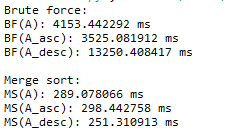
\includegraphics[scale=1.0]{./img/inversiones_PY.PNG}
  \caption{Resultados de la ejecución del programa inversiones.py (Hasta $N = 10^4$).}
  \label{fig:inversiones_PY}
\end{figure}

\subsection{Run your local machine the brute force and divide and conquer algorithms in C or C++ calculate the time for the first 10^5 numbers of size instance from Hackearth input and output and for the 10^5 sorted increasing and decreasing numbers.}

\begin{figure}[H]
  \centering
  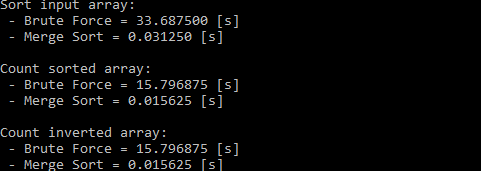
\includegraphics[scale=1.0]{./img/inversiones_C.PNG}
  \caption{Resultados de la ejecución del programa inversiones.c.}
  \label{fig:inversiones_C}
\end{figure}

\end{document}
